% !TeX TXS-program:bibliography = txs:///bibtex
%John M. Abowd and Lars Vilhuber
% $Id: report_on_SDS_2015.tex 1537 2015-05-01 23:20:30Z lv39 $
% $URL: https://forge.cornell.edu/svn/repos/ncrn-cornell/branches/papers/CNSTAT2015/text/report_on_SDS_2015.tex $
%%%%%%%%%%%%%%%%%%%%%%%%%%%%%%%%%%%%%%%
\documentclass[12pt,titlepage]{article}
%TCIDATA{OutputFilter=Latex.dll}
%------------ External info is stored in these files. Edit at your own risk ---
%++++++++++++++++++++ Adjust this as necessary ++++++++++++++++++++
%-------------------- Start of title info -------------------------
% Use these definitions, since they are also used in headers, PDF info,
% etc.

\input{titleinfo}


%--------------------


%%%%%%%%%%%%%%%%%%%%%%%%%%%%%%%%%%  %%

\date{\myversion
%\\ \vspace*{3em}{THIS VERSION PRELIMINARY AND INCOMPLETE: PLEASE DO NOT CITE}
}
%--------------------
\input{formats}
%--------------------
%try to eliminate the stupid * for \thanks in titlepage
\renewcommand\footnotemark{}
%--------------------
%----------------------
%To insert un-numbered footnotes (as on the title page)
%ref: http://en.wikibooks.org/wiki/LaTeX/Formatting#cite_note-csli_footnotes-0
\makeatletter
\def\blfootnote{\xdef\@thefnmark{}\@footnotetext}
\makeatother
%%%%%%%%%%%%%%%%%%%%%%%%%%%%%%%%%%%%%%%%%%%%%%%%%%%%%%%%%%%%%%%%%%%%%
%%%%%%%%%%%%%%%%%%%%%%%%%%%%%%%%%%%%%%%%%%%%%%%%%%%%%%%%%%%%%%%%%%%%%

% when ready, uncomment this line
%\excludecomment{instructions,constraint}
\excludecomment{instructions}

\title{\mytitle}
\author{\myauthorA \and \myauthorB}

\usepackage{Sweave}
\begin{document}
\input{report_on_SDS_2015-concordance}
\maketitle

 

 



\section{History of the Synthetic Data Server}
\input{history.tex}


\section{Access to the server}
\input{access.tex}

%\section{Validation}
%\input{validation.tex}

\section{Datasets}
\input{datasets.tex}

\section{Usage and impact}
After the Synthetic Data Server project was kicked off, account growth has been steady (see Figure~\ref{fig:accounts}).

\begin{figure}
\centering
\caption{Account creation and salient events\label{fig:accounts}}
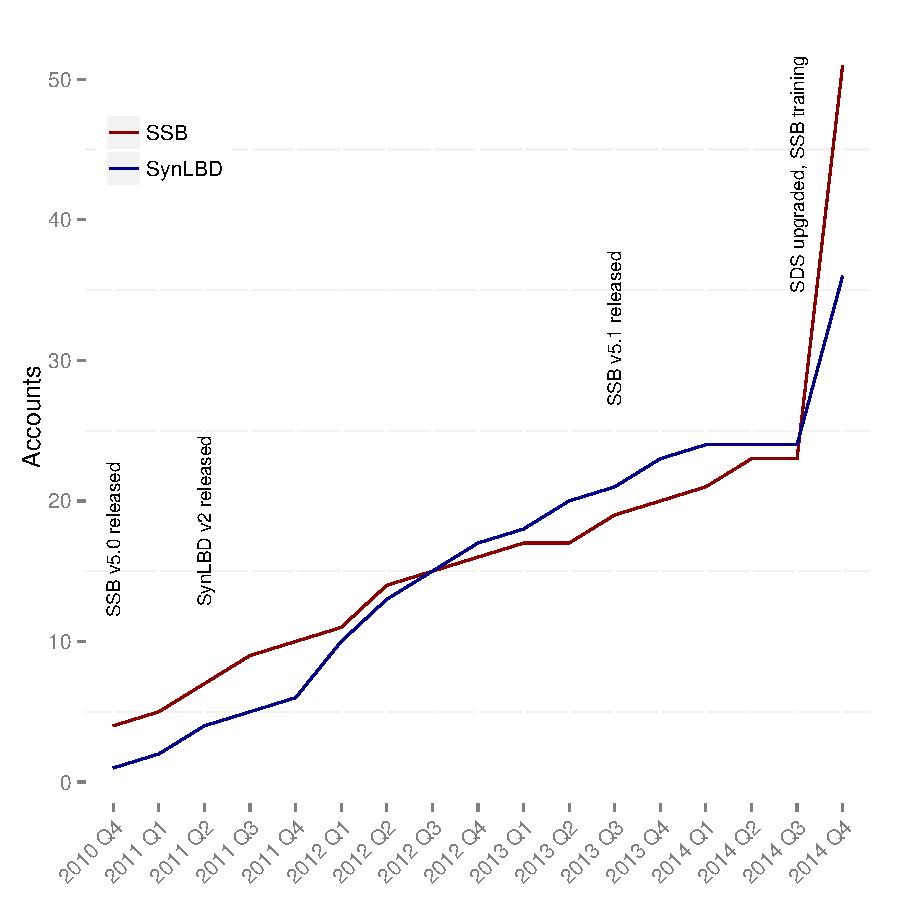
\includegraphics{report_on_SDS_2015-accounts}
\end{figure}


\subsection{Feedback loop}
Both of the current data providers have incorporated feedback from users into their data products. The \ac{SSB} with which the \ac{SDS} was launched was itself the second public iteration, after the original release of v4.0. The growth of the supporting IT infrastructure, first from its predecessor to the original instantiation of the \ac{SDS}, and subsequently in the 2014 IT upgrade mentioned earlier, reflected the growing interest that followed adaptations. In the case of the \ac{SSB}, such feedback first lead to the incorporation of additional variables in v5.1 \citep{SSB5.1}, and subsequently to further enhancements in v6.0 \citep{SSB6}. 
In the case of the \ac{SynLBD}, only one iteration has so far been released on the \ac{SDS}, but the key shortcomings in the structure of the SynLBD v2.0 \citep{SynLBD20} -- the absence of \ac{NAICS} codes, of any sort of geographic detail, and of indicators of firm structure -- have been reflected in the rejected access applications. 
As a reminder, access is granted when the technical requests are feasibly satisfied by the data on the \ac{SDS}. 
In the case of the SynLBD, we can quantify additional data requested that lead to applications being rejected. 
Out of 99 applications for access to the \ac{SynLBD} received through Jan 2015, 21 (21.21\%) were denied because they were not feasible using the synthetic data (this does not take into account applications that were partially feasible, which fall into the number of approvals). Of those denied, 
\begin{itemize}
\item 6 (28.57\%) had requested firm-level variables, 
\item 11 (52.38\%) had requested data to perform conditional geographic analysis, and
\item 1 (4.76\%) had requested data for specific \ac{NAICS} industries.
\end{itemize}
Such numbers, of course, do not take into account potential requestors that did not apply because a reading of the documentation revealed that the analysis was not feasible.

\subsection{Validation requests}
\input{validation.tex}
The last analysis of validation requests goes back to December 2012, and only for the \ac{SynLBD}. At the time, out of approximately 30 users, 3 had requested validation, and 2 of those had requested a second round of validation. [NEEDS updating] A common issue has been that users are unfamiliar with the constraints imposed by the validation procedure, in particular that all such validation requests are treated as an authorized release of results from an analysis of confidential data, and are thus subject to review by the Census Bureau's \ac{DRB}. In particular, the quantity of results requested surpasses not the ability of the confidential servers to compute, but rather is judged to be too high by the rules of the \ac{DRB}. 

\begin{figure}[htb]
\centering
\caption{From Bertrand et al (2015), their Figure~I}\label{fig:bertrand}
\begin{tabular}{cc}
(a) & (b)\\
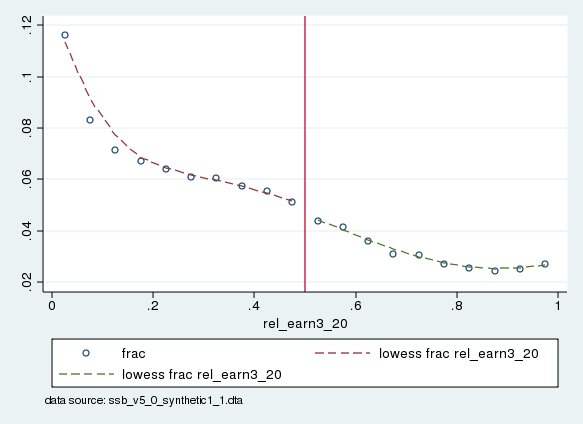
\includegraphics[width=0.4\textwidth]{jma_graph_rel_earn3_syn}&
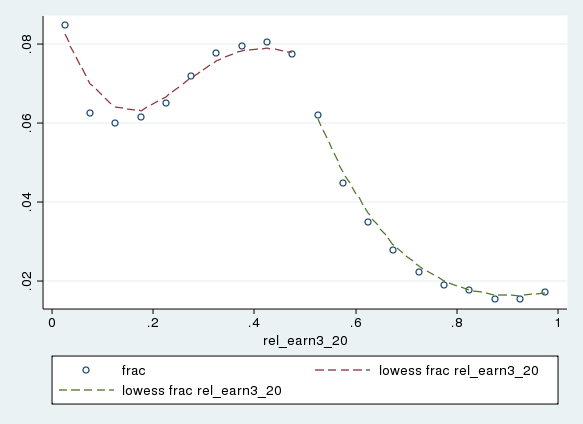
\includegraphics[width=0.4\textwidth]{jma_graph_rel_earn3}\\
\multicolumn{2}{l}{\tiny \it Note: See text for details on computation and provenance.}
\end{tabular}
\end{figure}

An example for a successful validation request combined with a cautionary note for users of the \ac{SSB} is illustrated by Figure~\ref{fig:bertrand}. In preparing \cite{Bertrand29012015}, the authors of that paper performed an analysis of the distribution of relative household income using a variety of datasets, including the \ac{SSB}. They obtained fairly robust results across a variety of datasets and time (see their Figure~III, reproduced here in Figure~\ref{fig:bertrand-qje-census}): there is a distinct break in the distribution of couples when the wife's income surpassed 50\%. However, the analysis with the \ac{SSB} produced a very different result, as illustrated in Figure~\ref{fig:bertrand}, Panel (a): there was no such break. The authors requested validation (which the Census Bureau was able to accomplish in a very short time), and the results obtained when their analysis was replicated against the confidential files yielded a different result, consistent with other datasets, as shown in Figure~\ref{fig:bertrand}, Panel (b), corresponding to their Figure~I. The ``success'' alluded to earlier is on both sides of the interaction. The researchers were able to very quickly ascertain that their model, when tested against the confidential data, yielded a publication-worth result. The Census Bureau, in exchange, obtained valuable feedback on the quality of the synthesis models, which they were able to take into account for the next iteration of the data production cycle. The cautionary note is that while useful for exploring the data and for testing models, not every model will yield valid results on the synthetic data.%
\footnote{We thank Marianne Bertrand for allowing us to use this example, and for kindly having provided the graphs for from the analyses using the \ac{GSF} and the \ac{SSB}.}


\begin{figure}[hbt]
\centering
\caption{From Bertrand et al (2015)}\label{fig:bertrand-qje-census}
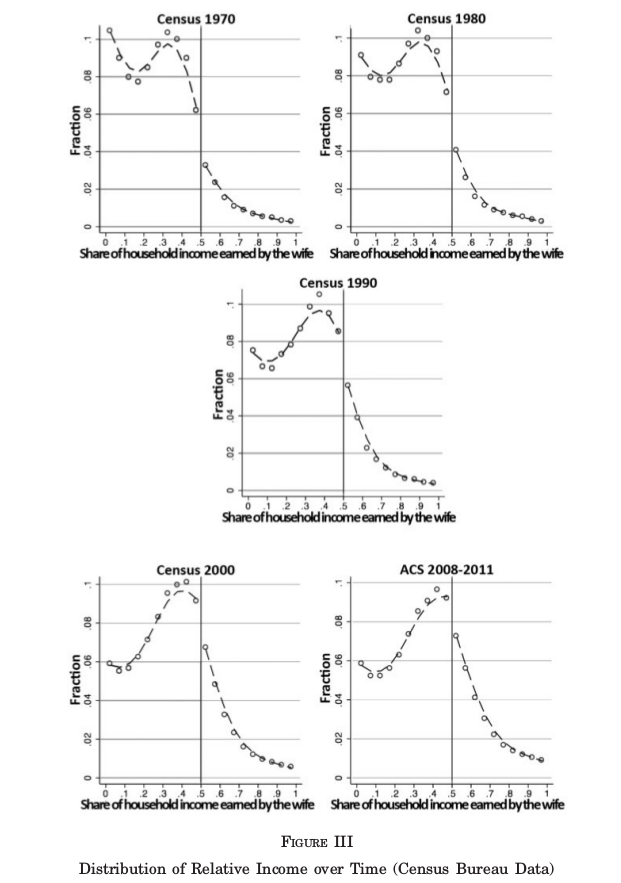
\includegraphics[width=0.5\textwidth]{Bertrand-QJE-2015-FigureIII}
\end{figure}


\subsection{Prior and subsequent experience in the Census RDC}



On 2014-10-14, we researched what kind of exposure users of the \ac{SDS} had had to confidential data at the Census Bureau, by investigating whether they had prior or subsequent Census RDC projects. Firgure~\ref{fig:rdcUse} summarizes the results.
Of the 106 users we identified in this way, 14 were Census internal users, i.e., users who were actively engaged in ongoing Census projects, presumably related to the validation exercises themselves. 
20 users were also present in some form in the Census RDC system. 11 users had been authorized for at least one RDC project prior to their access to the \ac{SDS}. 
More of interest, however, are the 3 users who obtained Census RDC access after their initial access to the \ac{SDS}, 
NA
We don't have firm evidence of the relationship between the RDC projects and the SDS project, but from personal conversations of the authors with presenters at RDC conferences, at least some of the RDC projects were direct continuation of SDS projects, in domains that were not covered by the synthetic data, but the analysis for which was prepared for on the \ac{SDS}. The average delay between project start on \ac{SDS} and project start on RDC projects for those projects that were authorized was 400 days.


\begin{figure}
\centering
\caption{Connection between Census RDC usage and Synthetic Data Server}\label{fig:rdcUse}
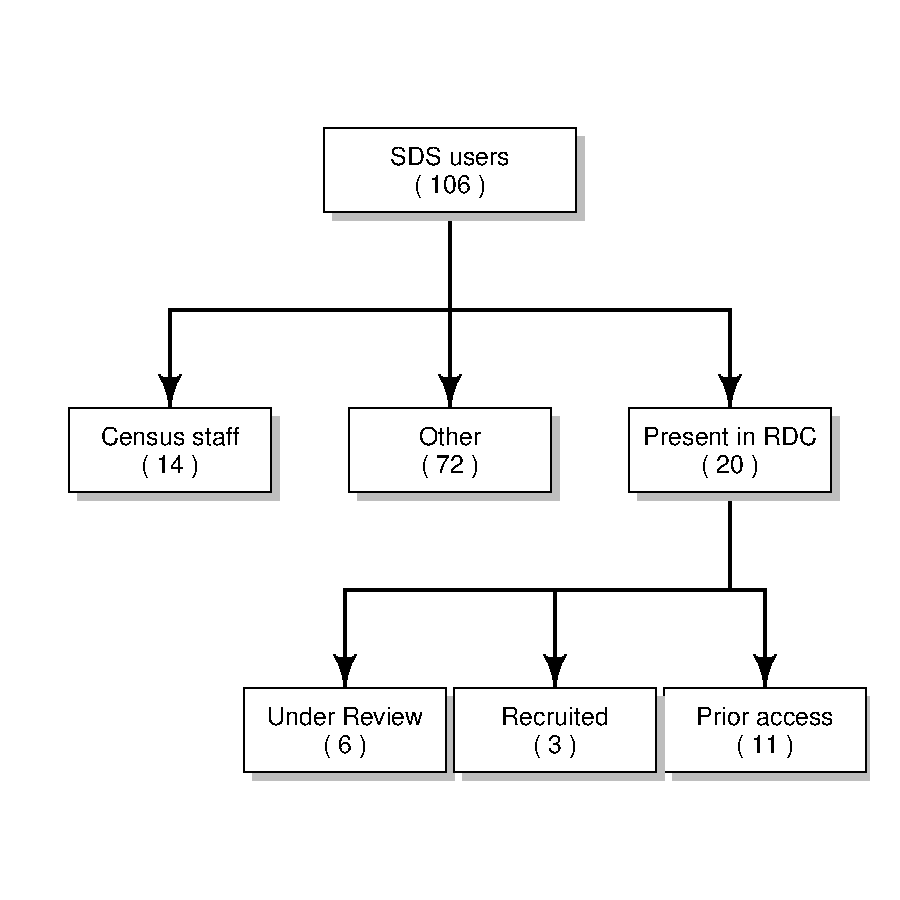
\includegraphics{report_on_SDS_2015-useRDCgraph}
\end{figure}


\section{Other activities}
\input{activities.tex}

\section{Bibliography}

A full and up-to-date bibliography can be found at \myhref{http://www2.vrdc.cornell.edu/news/synthetic-data-server/sds-bibliography}{the SDS website}.







\clearpage
\singlespacing
	% ------------------------------ Bibliography---------------------

	\bibliographystyle{\mybibstyle}
	\bibliography{../../docs/SDS_1042181.bib,../../docs/synlbd-data.bib,../../docs/synlbd-documents.bib,../../docs/ssb-data.bib,../../docs/ssb-documents.bib,../../docs/wsc2013.bib,../../docs/grants.bib}
	
	\section{Acronyms used}
	%TCIDATA{Version=5.00.0.2570}
%TCIDATA{LaTeXparent=0,0,sw-edit.tex}

% $Id: acronyms.tex 1720 2015-09-25 14:29:12Z lv39 $
% $URL: https://forge.cornell.edu/svn/repos/ncrn-cornell/branches/papers/PSD2014/text/acronyms.tex $
%
% Define acronyms to be used in the text here. See
% http://www.mackichan.com/index.html?techtalk/456.htm~mainFrame for usage in
% Scientific workplace context

\begin{acronym}
\acro{ACS}{American Community Survey} 
\acro{AHEAD}{Study of Assets and Health Dynamics Amongst the Oldest Old}
\acro{ASCII}{American Standard Code for Information  Interchange} %, typically used to denote raw text files in PC or Unix environments
\acro{ASM}{Annual Survey of Manufacturers}
\acro{BDS}{Business Dynamics Statistics}
\acro{BED}{Business Employment Dynamics}
\acro{BES}{Business Expenditure Survey}
\acro{BLS}{Bureau of Labor Statistics}
\acro{BRB}{Business Register Bridge}
\acro{BR}{Business Register}
\acro{CAC}{Cornell Center for Advanced Computing}
\acro{CBP}{County Business Patterns}
\acro{CBSA}{Core-Based Statistical Area}
\acro{CER}{Covered Earnings Records}
\acro{CES}{Center for Economic Studies}
\acro{CEW}{Covered Employment and Wages}%. Employment statistics program run by BLS in  conjunction with all states, also known as ES-202. Generally, when used  in this document, refers to public-use tabulations from the CEW, as  opposed to the confidential microdata received directly from the states.
\acro{CISER}{Cornell Institute for Social and Economic Research}
\acro{CIT}{Cornell Information Technologies}
\acro{CODA}{Children of Depression}
\acro{CPI}{Consumer Price Index}
\acro{CPI-U}{Consumer Price Index (All Urban Consumers)}
\acro{CPR}{Composite Person Record}
\acro{CPS}{Current Population Survey}
\acro{CRADC}{Cornell Restricted Access Data Center}
\acro{CTC}{Cornell Theory Center}
\acro{DCC}{Data Confidentiality Committee}
\acrodef{err}{excess reallocation rate}
\acrodef{jcr}{job creation rate}
\acrodef{jdr}{job destruction rate}
\acrodef{jrr}{job reallocation rate}
\acrodef{wrr}{worker reallocation rate}
\acro{DER}{Detailed Earnings Record}
\acro{DRB}{Disclosure Review Board}
\acro{DWS}{Displaced Worker Supplement}
\acro{ECF}{Employer Characteristics  File}
\acro{EHF}{Employment History Files}
\acro{EIN}{\acroextra{(federal) }Employer Identification Number}
\acro{ERR}{Excess Reallocation Rate}
\acro{ES-202}{ES-202\acroextra{. An older name for the \ac{QCEW} program}}
\acro{FHFA}{Federal Housing Finance Agency}
\acro{FIPS}{Federal information processing standards codes\acroextra{\ issued     by \ac{NIST}}}
\acro{FTI}{Federal Tax Information\acroextra{, typically covered under     Title 26, U.S.C.}}
\acro{GAL}{Geocoded Address List}
\acro{GIS}{Geographic Information System}
\acro{HPI}{House Price Index}
\acro{HRS}{Health and Retirement Study}
\acro{ICF}{Individual Characteristics File}
\acro{IRB}{Institutional Review Board}
\acro{IRS}{Internal Revenue Service}
\acro{ISR}{Institute for Social Research}
\acro{JCR}{Job Creation Rate}
\acro{JDR}{Job Destruction Rate}
\acro{JOLTS}{Job Openings and Labor Turnover Survey}
\acro{JRR}{Job Reallocation Rate}
\acro{LAUS}{Local Area Unemployment Statistics}
\acro{LBD}{Longitudinal Business Database}
\acro{LDB}{\ac{BLS}'s Longitudinal Business Database}
\acro{LED}{Local Employment Dynamics}
\acro{LEHD}{Longitudinal Employer-Household Dynamics}
\acro{LMI}{Labor Market Information}
\acro{MBR}{Master Beneficiary Record}
\acro{MEF}{Master Earnings File}
\acro{MER}{Master Earnings Record}
\acro{MLS}{Mass Layoff Statistics}
\acro{MMS}{Methodology, Measurement, and Statistics}
\acro{MN}{Minnesota}
\acro{MSA}{Metropolitan Statistical Area}
\acro{MSD}{Metropolitan Statistical Division}
\acro{MWR}{Multiple Worksite Report}
\acro{NAICS}{North American Industry Coding System}
\acro{NECTA}{New England  City and Town Area}
\acro{NIA}{National Institute on Aging}
\acro{NIST}{National Institute of Standards and Technology}
\acro{NLSY}{National Longitudinal Study of Youth}
\acro{NSF}{National Science Foundation}
\acro{NSTA}{NAICS SIC Treatment of Auxiliaries}
\acro{OTM}{OnTheMap}
\acro{PCF}{Person Characteristics File}
\acro{PHF}{Person History File}
\acro{PIK}{Protected Identity Key}
\acro{PSID}{Panel Study of Income Dynamics}
\acro{QCEW}{Quarterly Census of Employment and Wages\acroextra{, managed by   the \acf{BLS}}}
\acro{QWI}{Quarterly Workforce Indicators}
\acro{RDA}{Restricted Data Application}
\acro{RDC}{Research Data Center}
\acro{RUN}{Reporting unit number}
\acro{SEIN}{State employer identification number\acroextra{. It is     constructed from the state \ac{FIPS} code and the UI account     number. The BLS refers to the UI account number in combination with the     reporting unit number as SESA-ID}}
\acro{SEINUNIT}{SEIN reporting unit}
\acro{SEPB}{Summary of Earnings and Projected Benefits} % confidential SSA                                % file
\acro{SESA-ID}{State Employment Security Agency ID\acroextra{. The UI     account number in combination with the Reporting Unit Number is treated   as a unique establishment identifier.}}
\acro{SESA}{State Employment Security Agency}
\acro{SIC}{Standard Industry Classification}
\acro{SIPP}{Survey of Income and Program Participation}
\acro{SLID}{Survey of Labour and Income Dynamics}
\acro{SPF}{Successor-Predecessor File}
\acro{SRMI}{Sequential Regression Multiple Imputation}
\acro{SSA}{Social Security Administration}
\acro{SSI}{Supplemental Security Income}
\acro{SSN}{Social Security Number}
\acro{SSR}{Supplemental Security Record}
\acro{SynLBD}{Synthetic \ac{LBD}\acroextra{, a synthetic microdata file at the establishment level}}
\acro{U2W}{Unit-to-Worker Impute}
\acro{UI}{Unemployment Insurance}
\acro{WB}{War Babies}
\acro{WIA}{Workforce Investment Act}
\acro{WIB}{Workforce Investment Board}
\acro{WRR}{Worker Reallocation Rate}
\acro{WTS}{Windows Terminal Services}

% Usage in the later text:
%  \ac{acronym}         Expand and identify the acronym the first time; use
%                       only the acronym thereafter 
%  \acf{acronym}        Use the full name of the acronym.
%  \acs{acronym}        Use the acronym, even before the first corresponding
%                       \ac command 
%  \acl{acronym}        Expand the acronym without using the acronym itself.
\end{acronym}

%%% Local Variables: 
%%% mode: latex
%%% TeX-master: "proposal"
%%% End: 
 
	\newpage
\tableofcontents

% Appendix
%\clearpage
%\appendix
%\part*{APPENDIX}
%\addcontentsline{toc}{part}{Appendix} 
%\setcounter{section}{0}
%\label{sec:appendix}
%% $Id: appendix.tex 1720 2015-09-25 14:29:12Z lv39 $
\appendix
\section*{Appendix}
\subsection*{Acronyms}
%TCIDATA{Version=5.00.0.2570}
%TCIDATA{LaTeXparent=0,0,sw-edit.tex}

% $Id: acronyms.tex 1720 2015-09-25 14:29:12Z lv39 $
% $URL: https://forge.cornell.edu/svn/repos/ncrn-cornell/branches/papers/PSD2014/text/acronyms.tex $
%
% Define acronyms to be used in the text here. See
% http://www.mackichan.com/index.html?techtalk/456.htm~mainFrame for usage in
% Scientific workplace context

\begin{acronym}
\acro{ACS}{American Community Survey} 
\acro{AHEAD}{Study of Assets and Health Dynamics Amongst the Oldest Old}
\acro{ASCII}{American Standard Code for Information  Interchange} %, typically used to denote raw text files in PC or Unix environments
\acro{ASM}{Annual Survey of Manufacturers}
\acro{BDS}{Business Dynamics Statistics}
\acro{BED}{Business Employment Dynamics}
\acro{BES}{Business Expenditure Survey}
\acro{BLS}{Bureau of Labor Statistics}
\acro{BRB}{Business Register Bridge}
\acro{BR}{Business Register}
\acro{CAC}{Cornell Center for Advanced Computing}
\acro{CBP}{County Business Patterns}
\acro{CBSA}{Core-Based Statistical Area}
\acro{CER}{Covered Earnings Records}
\acro{CES}{Center for Economic Studies}
\acro{CEW}{Covered Employment and Wages}%. Employment statistics program run by BLS in  conjunction with all states, also known as ES-202. Generally, when used  in this document, refers to public-use tabulations from the CEW, as  opposed to the confidential microdata received directly from the states.
\acro{CISER}{Cornell Institute for Social and Economic Research}
\acro{CIT}{Cornell Information Technologies}
\acro{CODA}{Children of Depression}
\acro{CPI}{Consumer Price Index}
\acro{CPI-U}{Consumer Price Index (All Urban Consumers)}
\acro{CPR}{Composite Person Record}
\acro{CPS}{Current Population Survey}
\acro{CRADC}{Cornell Restricted Access Data Center}
\acro{CTC}{Cornell Theory Center}
\acro{DCC}{Data Confidentiality Committee}
\acrodef{err}{excess reallocation rate}
\acrodef{jcr}{job creation rate}
\acrodef{jdr}{job destruction rate}
\acrodef{jrr}{job reallocation rate}
\acrodef{wrr}{worker reallocation rate}
\acro{DER}{Detailed Earnings Record}
\acro{DRB}{Disclosure Review Board}
\acro{DWS}{Displaced Worker Supplement}
\acro{ECF}{Employer Characteristics  File}
\acro{EHF}{Employment History Files}
\acro{EIN}{\acroextra{(federal) }Employer Identification Number}
\acro{ERR}{Excess Reallocation Rate}
\acro{ES-202}{ES-202\acroextra{. An older name for the \ac{QCEW} program}}
\acro{FHFA}{Federal Housing Finance Agency}
\acro{FIPS}{Federal information processing standards codes\acroextra{\ issued     by \ac{NIST}}}
\acro{FTI}{Federal Tax Information\acroextra{, typically covered under     Title 26, U.S.C.}}
\acro{GAL}{Geocoded Address List}
\acro{GIS}{Geographic Information System}
\acro{HPI}{House Price Index}
\acro{HRS}{Health and Retirement Study}
\acro{ICF}{Individual Characteristics File}
\acro{IRB}{Institutional Review Board}
\acro{IRS}{Internal Revenue Service}
\acro{ISR}{Institute for Social Research}
\acro{JCR}{Job Creation Rate}
\acro{JDR}{Job Destruction Rate}
\acro{JOLTS}{Job Openings and Labor Turnover Survey}
\acro{JRR}{Job Reallocation Rate}
\acro{LAUS}{Local Area Unemployment Statistics}
\acro{LBD}{Longitudinal Business Database}
\acro{LDB}{\ac{BLS}'s Longitudinal Business Database}
\acro{LED}{Local Employment Dynamics}
\acro{LEHD}{Longitudinal Employer-Household Dynamics}
\acro{LMI}{Labor Market Information}
\acro{MBR}{Master Beneficiary Record}
\acro{MEF}{Master Earnings File}
\acro{MER}{Master Earnings Record}
\acro{MLS}{Mass Layoff Statistics}
\acro{MMS}{Methodology, Measurement, and Statistics}
\acro{MN}{Minnesota}
\acro{MSA}{Metropolitan Statistical Area}
\acro{MSD}{Metropolitan Statistical Division}
\acro{MWR}{Multiple Worksite Report}
\acro{NAICS}{North American Industry Coding System}
\acro{NECTA}{New England  City and Town Area}
\acro{NIA}{National Institute on Aging}
\acro{NIST}{National Institute of Standards and Technology}
\acro{NLSY}{National Longitudinal Study of Youth}
\acro{NSF}{National Science Foundation}
\acro{NSTA}{NAICS SIC Treatment of Auxiliaries}
\acro{OTM}{OnTheMap}
\acro{PCF}{Person Characteristics File}
\acro{PHF}{Person History File}
\acro{PIK}{Protected Identity Key}
\acro{PSID}{Panel Study of Income Dynamics}
\acro{QCEW}{Quarterly Census of Employment and Wages\acroextra{, managed by   the \acf{BLS}}}
\acro{QWI}{Quarterly Workforce Indicators}
\acro{RDA}{Restricted Data Application}
\acro{RDC}{Research Data Center}
\acro{RUN}{Reporting unit number}
\acro{SEIN}{State employer identification number\acroextra{. It is     constructed from the state \ac{FIPS} code and the UI account     number. The BLS refers to the UI account number in combination with the     reporting unit number as SESA-ID}}
\acro{SEINUNIT}{SEIN reporting unit}
\acro{SEPB}{Summary of Earnings and Projected Benefits} % confidential SSA                                % file
\acro{SESA-ID}{State Employment Security Agency ID\acroextra{. The UI     account number in combination with the Reporting Unit Number is treated   as a unique establishment identifier.}}
\acro{SESA}{State Employment Security Agency}
\acro{SIC}{Standard Industry Classification}
\acro{SIPP}{Survey of Income and Program Participation}
\acro{SLID}{Survey of Labour and Income Dynamics}
\acro{SPF}{Successor-Predecessor File}
\acro{SRMI}{Sequential Regression Multiple Imputation}
\acro{SSA}{Social Security Administration}
\acro{SSI}{Supplemental Security Income}
\acro{SSN}{Social Security Number}
\acro{SSR}{Supplemental Security Record}
\acro{SynLBD}{Synthetic \ac{LBD}\acroextra{, a synthetic microdata file at the establishment level}}
\acro{U2W}{Unit-to-Worker Impute}
\acro{UI}{Unemployment Insurance}
\acro{WB}{War Babies}
\acro{WIA}{Workforce Investment Act}
\acro{WIB}{Workforce Investment Board}
\acro{WRR}{Worker Reallocation Rate}
\acro{WTS}{Windows Terminal Services}

% Usage in the later text:
%  \ac{acronym}         Expand and identify the acronym the first time; use
%                       only the acronym thereafter 
%  \acf{acronym}        Use the full name of the acronym.
%  \acs{acronym}        Use the acronym, even before the first corresponding
%                       \ac command 
%  \acl{acronym}        Expand the acronym without using the acronym itself.
\end{acronym}

%%% Local Variables: 
%%% mode: latex
%%% TeX-master: "proposal"
%%% End: 

%\clearpage


\section*{Additional tables}
\begin{table}
\caption{Suppressions in firm-level BDS\label{tab:bds_f}}
\centering
\begin{tabular}{lcrr}\hline%
&&\bfseries No. of&\bfseries Percent\\
\bfseries Type & \bfseries Level & \bfseries  cells
& \bfseries  suppressed\\
\hline
\\
\csvreader[head to column names]%
{programs/bds_f_suppressions.csv}{}%
{\type & \level & \cells & \percentsup\\}%
\\\hline
\multicolumn{4}{p{0.5\textwidth}}{\footnotesize Note: Cells are year $x$ categories, where the 
number of categories varies by published table.}

\end{tabular}
\end{table}


\end{document}

